\chapter{Container-Runtimes}
\label{chap:compCtnrRuntimes}

Container-Runtimes sind das Herz eines jeden Container-Angebots. Sie instanziieren übergebene Prozesse in isolierten Containern. In diesem Kapitel werden verschiedene Runtimes miteinander verglichen und veranschaulicht, wie Runtimes neben Docker für spezielle Anforderungen besser geeignet sind.

\section{Vorgehen}
\label{sec:vorgehen}
Um verschiedene Runtimes zu vergleichen wurde eine eigene Anwendung mit drei Microservices implementiert. Dabei wurden, wie in \fref{fig:todosStack} zu sehen, verschiedene Technologien verwendet, um zu prüfen, wie die getesteten Container-Runtimes mit diesen umgehen. Diese wurde im Folgenden mit verschiedenen Runtimes bereitgestellt.

\begin{figure}[h]
	\begin{center}
		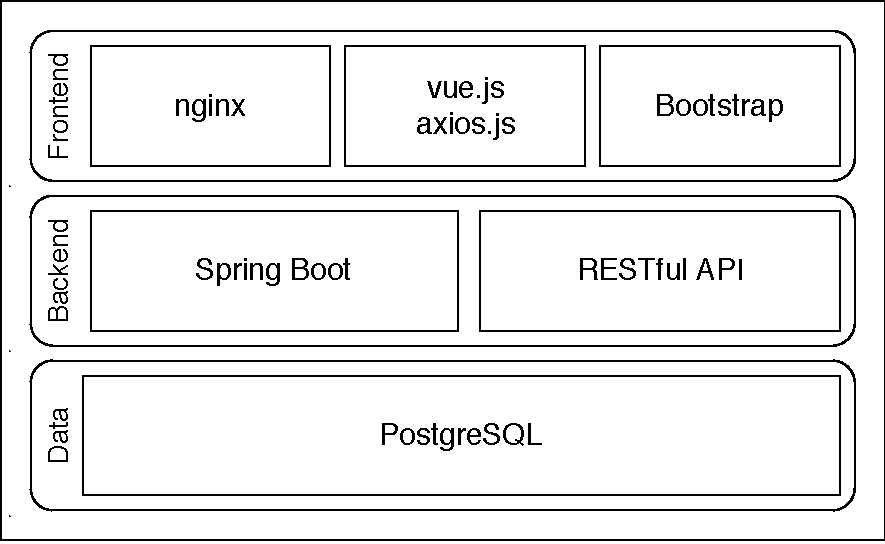
\includegraphics[width=0.7\textwidth]{bilder/microservice-example-stack.pdf}
		\caption{Beispielhafte Darstellung einer Micorservice-Architektur}
		\label{fig:todosStack}
	\end{center}
\end{figure}

\section{Docker Stack}
\label{sec:compDocker}
Docker ist der de facto Standard unter den Container-Technologien und bietet eine vollständige Plattform zur Verwaltung und Orchestrierung von Container (Docker Swarm), der Verbreitung von \glspl{gls-image} (Docker Hub bzw. Docker Store) und der Verwaltung des Container-Lifecycles (Docker CLI) an.

\begin{figure}[h]
	\begin{center}
		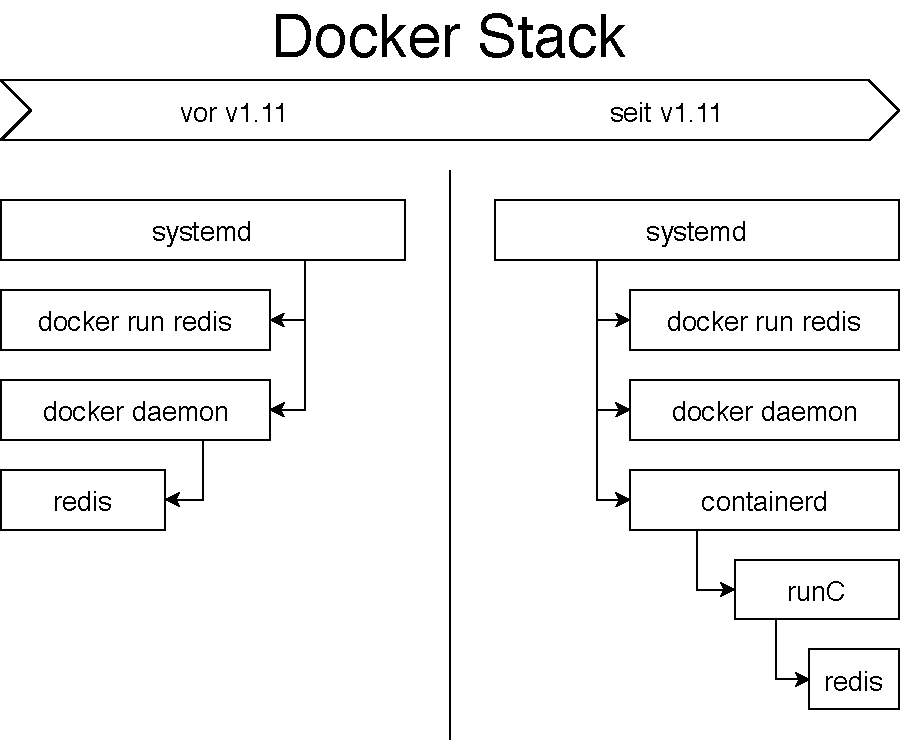
\includegraphics[width=0.9\textwidth]{bilder/docker-stack-containerd-runc.pdf}
		\caption{Docker Stack \citep{RktVsOtherProjects}}
		\label{fig:dockerStack}		
	\end{center}
\end{figure}

Dabei kommen innerhalb des Docker Stacks die Runtimes \texttt{runc} und \texttt{containerd} zum Einsatz. Durch die in \fref{fig:dockerStack} gezeigte Abkapselung der Runtime kann Docker auf jede beliebige \gls{acr-oci}-konforme Runtime aufbauen. Der dadurch gewonnene Vorteil der Kompatibilität bietet allerdings auch Nachteile. Falls einer der vielen Komponenten im Container-Stack einen Bug aufweist, ist das Debugging der Anwendung deutlich komplexer und Fehler können langsamer gefunden werden. Zudem benötigt der Docker-Daemon privilegierte Berechtigungen um die in \fref{sec:funktionsweise} beschriebenen Konzepte zu Nutzen. Da der Daemon auch für den Download und Bau-Prozess der Images zuständig ist, werden alle Images in Docker im Kontext des Users \texttt{root} erstellt.

\subsection{Vorgehensweise}
\label{sec:compDockerVorgehen}

Um den beispielhaften Microservice aus \fref{fig:todosStack} zu Container wurde zuerst für jeden Service ein Image erstellt und diese dann in Containern gestartet. Um dieses Vorgehen zu erleichtern wurde danach \texttt{docker-compose} genutzt, um alle Container in einer Datei zu spezifizieren. Folgend werden beide Wege genauer beschrieben und Vor- bzw. Nachteile dieser Vorgehensweisen aufgezeigt.

Docker verwendet zur Beschreibung eines Images das Dockerfile. Dieses verwendet spezifische Keywords, um Docker beim Bau eines Images zu steuern (\fref{lst:dockerfileExmpl}).

\begin{listing}[h]
	\begin{minted}[breaklines]{dockerfile}
FROM nginx:1.13-alpine
VOLUME /tmp
ADD ./index.html /usr/share/nginx/html/index.html
EXPOSE 80
ENTRYPOINT ["nginx","-g","daemon off"]
	\end{minted}
	\caption{Beispiel für ein Dockerfile}
	\label{lst:dockerfileExmpl}
\end{listing}

Dabei wird deklariert, von welchen Baseimage das neue Image erzeugt werden soll (\textbf{FROM}), welche Änderungen an diesem Image vorgenommen werden müssen (\textbf{VOLUME, ADD, EXPOSE}) und welchen Prozess der Container Isolieren soll (\textbf{ENTRYPOINT}). Dieses Vorgehen erlaubt es einfach, neue Container auf Basis andere zu erzeugen und diese für Dritte zu Verfügung zu stellen. Zu diesem Zweck bietet Docker den Docker Hub an, der als Standardrepository im Docker Stack verwendet wird. Dieser hostet mittlerweile mehr als 100 offizielle Images und eine Vielzahl von Images, die aus der wachsenden Docker Community kommen. Um die in \fref{fig:todosStack} gezeigte Anwendung zu Containern benötigt man somit drei Dockerfiles. Nach dem anlegen der Dockerfiles kann mit dem Befehl \mintinline[breaklines]{bash}{docker build -t <name of image>:<version of image> <path to dockerfile>} das entsprechende Image erstellt werden. Diese Images können mit \mintinline[breaklines]{bash}{docker run <name of image>:<version of image>} containerisiert werden. Durch diesen Prozess kann die gesamte in \fref{fig:todosStack} gezeigte Anwendung in wenigen Minuten gestartet werden.

Vereinfacht wird dieser Prozess mit dem Tool \texttt{docker compose}. Dieses erlaubt es in einer \gls{acr-yml}-Datei alle benötigten Container Images zu spezifizieren und mit dem Befehl \mintinline{bash}{docker-compose up} zu starten (siehe \fref{lst:dockerComposeTodos}).

\begin{listing}[h]
	\begin{minted}[breaklines]{yaml}
version: '3'
services:
 data:
  image: library/postgres
  environment:
   POSTGRES_USER: docker
   POSTGRES_PASSWORD: docker
   POSTGRES_DB: todos
 back:
  build:
   context: ./backend
   ports:
    - "8080:8080"
   environment:
    POSTGRES_PORT: 5432
    POSTGRES_IP: data
 front:
  image: nginx:latest
  ports:
   - "80:80"
  volumes:
   - ./frontend:/usr/share/nginx/html
	\end{minted}
	\caption{docker-compose.yaml für Micorservices}
	\label{lst:dockerComposeTodos}
\end{listing}

Der größte Unterschied liegt dabei in der Art und Weise, wie Container innerhalb des Compose-Clusters angesprochen werden können. Jeder Container bekommt zu seiner IP einen DNS Eintrag mit dem Namen des Service im docker-compose.yml. Dadurch lassen sich die Services einfacher miteinander verknüpfen, da die IP des Containers nicht bekannt sein muss.

\subsection{Bewertung}
\label{sec:compDockerBewertung}
Docker erlaubt es einfach, den Service in Containern bereitzustellen. Dafür ist vor allem die große Auswahl bereits bestehender Images verantwortlich, aber auch die einfache Nutzung durch Docker Compose. Das Imageformat für Dockerfiles ist zwar einfach, aber grade für Unixsysteme ungewöhnlich und nur mit Dokumentation nutzbar. Die Vorteile der einfachen Nutzung kommen allerdings zu einem Preis: Sicherheit. Images auf dem Dockerhub sind nicht verifizierbar, können somit Schadware und Sicherheitsprobleme mit sich bringen. Zudem baut Docker jedes Image unter dem Nutzer root, wodurch potentielle Sicherheitsrisiken, wie falsch konfigurierte AppArmor Profile, nicht beim Bau-Prozess auffallen. Viele dieser Probleme kommen durch die in \fref{fig:dockerStack} gezeigte Architektur, bei der die Docker-\gls{acr-cli} nur ein Client ist, der den Docker Daemon steuert. Diese Herangehensweise erlaubt auch kaum Integration mit bereits vorhandenen Linux Tools wie \texttt{systemd} oder \texttt{upstart}.

\todo{Image share mit Docker Hub, private Repos für Firmen, Integration mit Orchestatoren}

\section{rkt}
\label{sec:compRkt}

CoreOS veröffentlicht mit rkt den aktuell größten Konkurrenten zu Docker. Dieser setzt, wie in \fref{fig:rktProcessModell} zu sehen, auf ein deutlich vereinfachtes Prozessmodell. Diese ist deutlich linuxartiger, wodurch rkt im Vergleich zu Docker sicherer ist. Zudem ist rkt auf die Integration mit \texttt{systemd} konzipiert, wodurch sich der Container von diesem Überwachen und steuern lässt.

\begin{figure}[h]
	\begin{center}
		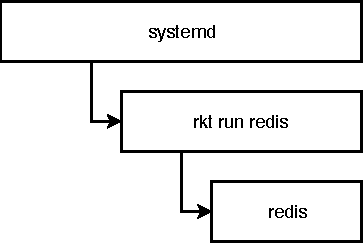
\includegraphics[scale=0.9]{bilder/rkt-process.pdf}
		\caption{rkt Prozess Modell \citep{RktVsOtherProjects}}
		\label{fig:rktProcessModell}		
	\end{center}
\end{figure}


\subsection{Vorgehensweise}
\label{sec:compRktVorgehen}

Im Gegensatz zu Docker bietet rkt die Möglichkeit verschiedene Imageformate zu nutzen um Container zu erstellen. Neben dem Dockerformat können auch OCI-konforme Bundles und \glspl{acr-aci} ausgeführt werden. Um den beispielhaften Microservice aus \fref{fig:todosStack} bereitzustellen, wurde für jeden Service ein \gls{acr-aci} erstellt. Zu diesem Zweck wird das Tool \texttt{acbuild} benötigt, welches ähnlich dem Syntax eines Dockerfiles einzelne Befehle hat um das zu erstellende \gls{acr-aci} zu spezifizieren (siehe \fref{lst:acbuildCommands}). Ein Container mit dem daraus resultierenden \gls{acr-aci} kann mit dem Befehl \mintinline[breaklines]{bash}{systemd-run rkt run --insecure-options=image nginx-latest-linux-amd64.aci} gestartet werden.

\begin{listing}[h]
	\begin{minted}[breaklines]{bash}
acbuild --debug begin

acbuildEnd() {
	export EXIT=$?
	acbuild --debug end && exit $EXIT 
}
trap acbuildEnd EXIT

acbuild --debug set-name example.com/nginx
acbuild --debug dep add quay.io/coreos/alpine-sh
acbuild --debug run apk update
acbuild --debug run apk add nginx
acbuild --debug port add http tcp 80
acbuild --debug mount add html /usr/share/nginx/html
acbuild --debug set-exec -- /usr/sbin/nginx -g "daemon off;"
acbuild --debug write --overwrite nginx-latest-linux-amd64.aci
	\end{minted}
	\caption{Bash Script um \gls{acr-aci} mit \texttt{acbuild} zu erstellen \citep{AppContainer}}
	\label{lst:acbuildCommands}
\end{listing}

Dabei fallen folgende Unterschiede zur Herangehensweise mit Docker auf:
\begin{enumerate}
	\item \texttt{systemd-run} \\ 
	Dieses Prefix wird benötigt um einen rkt Container im Hintergrund auszuführen, vergleichbar mit \texttt{docker run -d <image>}. Da rkt kein Daemon nutzt (siehe \fref{fig:rktProcessModell}), kann es mit bekannten und verbreiteten Linux Tools genutzt werden kann. Um den Container-Prozess zu überwachen und zu steuern wird das Initsystem \texttt{systemd} verwendet.
	\item \texttt{--insecure-options=image} \\
	rkt verlangt bei jedem Image, dass es von einer vertrauenswürdigen Quelle gebaut wurde. Dazu nimmt rkt an, dass jeder Image digital signiert ist. Da dies bei dem angelegten \gls{acr-aci} nicht der Fall ist, kann dieses Verhalten mit der gegebenen Option ausgeschaltet werden.
\end{enumerate}

Um Container miteinander zu verknüpfen nutzt rkt das von der \gls{acr-cncf} publizierte \gls{acr-cni}. Dieses erlaubt es, mittels einer JSON-Konfiguration, neue Routen für den Traffic zum Container zu spezifizieren (siehe \fref{lst:cniConfig}). Dadurch kann man, ähnlich wie bei Docker Compose, einzelnen Containern DNS Namen zuweisen und somit ohne das wissen der IP Container verknüpfen.

\begin{listing}[h]
	\begin{minted}[breaklines]{json}
{
	"cniVersion": "0.2.0",
	"name": "mynet",
	"type": "bridge",
	"bridge": "cni0",
	"isGateway": true,
	"ipMasq": true,
	"ipam": {
		"type": "host-local",
		"subnet": "10.22.0.0/16",
		"routes": [
			{ "dst": "0.0.0.0/0" }
		]
	}
}
	\end{minted}
	\caption{Beispielhafte \gls{acr-cni}-Konfiguration}
	\label{lst:cniConfig}
\end{listing}

\subsection{Bewertung}
\label{sec:compRktBewertung}
In vielen Punkten gleichen sich rkt und Docker. Bei beiden steht das bereitstellen einer Anwendung im Mittelpunkt. Doch gerade was das Thema Sicherheit und die Linuxähnlichkeit angeht treffen unterschiedliche Ansätze aufeinander. CoreOS bewegt sich näher an dem für Linuxsysteme typischen Aufbau und bietet mit rkt Integrationen zu weitverbreiteten Tools wie \texttt{systemd} an. Zudem benötigt rkt keine privilegierten Berechtigungen und arbeitet vollständig im Nutzerkontext. Durch dieses Vorgehen ist eine Privilege-Escalation weniger wahrscheinlich. Zudem lässt sich der rkt Prozess granularer Steuern, da er keinen Daemon nutzt. Diese Vorteile kommen allerdings zum Preis von mehr Konfigurationsaufwand. Wenn man \fref{lst:dockerfileExmpl} und \fref{lst:acbuildCommands} vergleicht wird man feststellen, dass das erstellen von Images mit \texttt{acbuild} komplexer und aufwändiger ist. Zudem wird neben rkt das Tool \texttt{acbuild} benötigt, da rkt selber keine Images erstellen kann, sondern lediglich eine Runtime bietet. Weiterreichend ist die Konfiguration des Netzwerks mittels \gls{acr-cni} umfangreicher und komplexer. 
\todo{Image share via https Webserver, keine notwendigkeit für Config von priv Repos, Integration mit Kubernetes, ...}

\section{LXD / LXC}
\label{sec:compLXD}

\begin{itemize}
	\item Gedacht für volle Linux Distros, nicht unbedingt Apps
	\item in Verbindung mit Docker, statt direkte Konkurenz
	\item LXD = LXC + RESTful API
	\item Docker bis anfang 2014 based of LXC
	\item komplexer zu nutzen, da lower Level
	\item Network zwischen Containern nur mit Linux mitteln, wissen von Nöten
	\item Betroffen von Linux-Kernel issues, keine Abstarktion
	\item RESTful API nutzbar über Netz, steuerung ohne SSH, Access zu VM, ...
\end{itemize}

\section{runc}
\label{sec:compRunc}

\begin{itemize}
	\item OCI stdimpl
	\item Low Level
	\item OCI bundles, mehrere Dateien zur Steuerung (config json, rootfs tar)
	\item Trend zu std, docker impl
	\item keine Versicherung durch Signatur / Verschlüsselung
	\item CRI-O für Kubernets
\end{itemize}

\section{VM basierte Runtimes}
\label{sec:compVMbased}

Notes:
\begin{itemize}
	\item Mehr sicherheit, seperation Kernel
	\item Weniger Performance, Einzelne Aufrufe, starten und stoppen, ... "teurer" 
	\item Erklären KataContaienrs, gVisor (neue Runtime)
\end{itemize}

\section{Fazit}
\label{sec:compFazit}